%!TEX root = ../TAMUTemplate.tex
%%%%%%%%%%%%%%%%%%%%%%%%%%%%%%%%%%%%%%%%%%%%%%%%%%%
%
%  New template code for TAMU Theses and Dissertations starting Fall 2016.
%
%  Author: Sean Zachary Roberson 
%	 Version 3.08.16
%  Last updated 8/19/2016
%
%%%%%%%%%%%%%%%%%%%%%%%%%%%%%%%%%%%%%%%%%%%%%%%%%%%

%%%%%%%%%%%%%%%%%%%%%%%%%%%%%%%%%%%%%%%%%%%%%%%%%%%%%%%%%%%%%%%%%%%%%%
%%                           SECTION I
%%%%%%%%%%%%%%%%%%%%%%%%%%%%%%%%%%%%%%%%%%%%%%%%%%%%%%%%%%%%%%%%%%%%%


\pagestyle{plain} % No headers, just page numbers
\pagenumbering{arabic} % Arabic numerals
\setcounter{page}{1}


\chapter{\uppercase {Introduction}}

Since the mid-1970s, the Standard Model (SM) of particle physics has been the leading theory describing three of the four known fundamental forces (not including gravity) as well as classifying all of the known elementary particles.
In 1961 Sheldon Glashow combined the electromagnetic and weak interactions in the first step towards creating the SM~\cite{GLASHOW1961579}.
Steven Weinberg and Abdus Salam~\cite{PhysRevLett.19.1264,salam} continued this work by adding in the Higgs mechanism~\cite{PhysRevLett.13.321,PhysRevLett.13.508,PhysRevLett.13.585} (more on this later) in 1967.
The model entered its current form in 1973-1974 whith the introduction of the strong force and quantum chromodynamics.
The model can be broken down into the matter particles, spin $\frac{1}{2}$ fermions called leptons and quarks, the force mediators, spin 1 gauge bosons, and the spin-0 mediator of the Higgs field, all of which can be found in figure~\ref{fig:standard_model}.
Even during it's formative years, the SM's success at predicting new particles (i.e. the top quark in 1995) and describing the properties of known particles (i.e. $W^{\pm}$ to $Z^{0}$ mass ratio) is undeniable.
However, the model was left incomplete until July 4th, 2012 when the long predicted Higgs boson (H) was discovered by both the ATLAS~\cite{20121} and CMS~\cite{201230} experiments.
It took almost 50 years for experimentalists to confirm the existence of the boson first proposed in 1964 to give mass to itself and all of the other massive particles through the process of electroweak symmetry breaking.

\begin{figure}[!hbt]
	%\scalebox{.45}{\input{StandardModel}}
	\centering
	\resizebox{0.65\textwidth}{!}{\input{StandardModel}}
	\caption{The Standard Model of particle physics. The model includes three generations of matter particles (leptons and quarks) as well as the gauge and Higgs bosons.}
	\label{fig:standard_model}
\end{figure}

Using 19.6\fbinv of 8\tev data from the Compact Muon Solenoid (CMS) experiment at CERN, the Higgs boson mass was measured to be \longmass{125.7}{0.3}{0.3}{\gev} by five major decay modes: $H\rightarrow\gamma\gamma$, $H\rightarrow\tau\tau$, $H\rightarrow{bb}$, $H\rightarrow{ZZ}$, and $H\rightarrow{WW}$~\cite{CMS-PAS-HIG-13-005}.
Since then, the experiment has entered a phase of intense study of the new particle.
Every property of the new boson and all of its decay channels must be studies in great detail to confirm that it is indeed the SM Higgs boson and not a very similar particle.
Additionally, any deviation from the SM predictions could point to some new, as yet unexplored physics.

To this end this analysis will use the \HWWlnujj decay channel to search for the Higgs boson.
Although the \HWWlnujj channel was used in the original combined limit, the previous search was not sensitive to the ``low mass'' Higgs, but only to a $\MH>170\gev$.

\begin{figure}[!hbt]
	\centering
	\begin{subfigure}[t]{0.54\textwidth}
		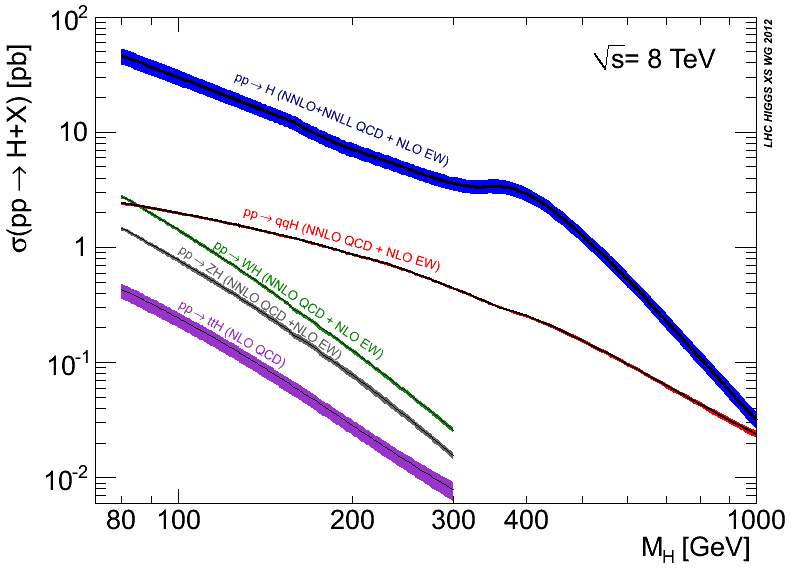
\includegraphics[width=\textwidth]{\figpath/Chapter1/Higgs_XS_8TeV.png}
		\label{fig:CERN_accelerator_complex}
	\end{subfigure}
	\begin{subfigure}[t]{0.41\textwidth}
		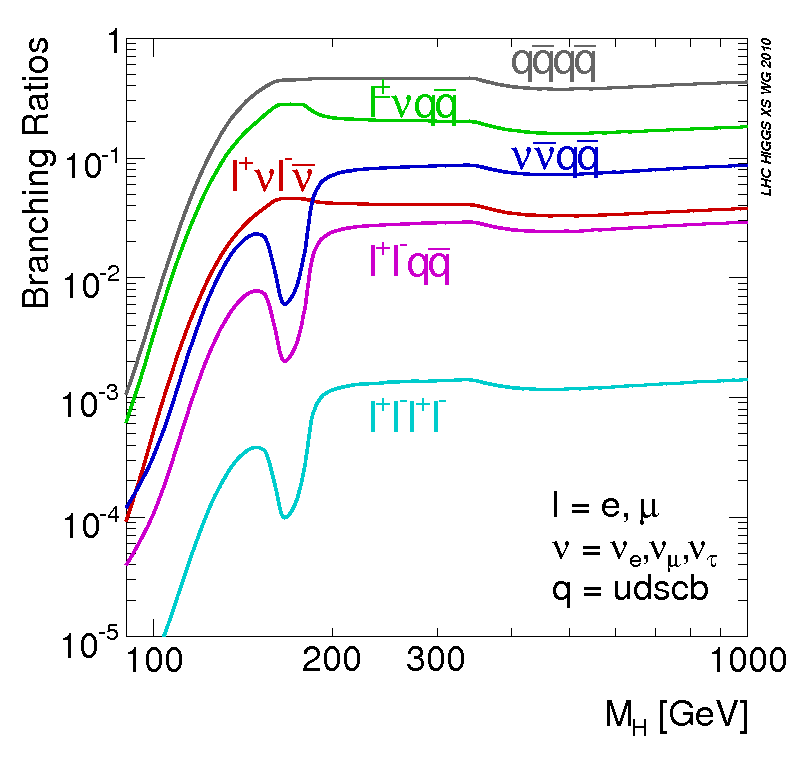
\includegraphics[width=\textwidth]{\figpath/Chapter1/Higgs_BR_4fermion.png}
		\label{fig:LHC_LEP_injection_complex}
	\end{subfigure}
	\caption{The Standard Model Higgs production cross sections at 8\tev (left) and branching ratios to four fermion final states (right).}
	\label{fig:Higgs_XS_and_BR}
\end{figure}



\begin{comment}
LHC & CMS
The discovery of the Higgs boson was one of the primary motivators behind the conception and construction of the Large Hadron Collider (LHC) and its two multi-purpose experiments, CMS and ATLAS. 


Objects and PF
ME
Analysis
Expected Limits




Aysen
=====
The Standard Model (SM) of particle physics is a theory that summarizes our
current knowledge about the most fundamental constituents of matter and interac- tions between them. The Higgs boson is a central part of the SM as it provides masses to all other particles. After many decades of searches for it, on the 4th of July 2012 CERN announced a discovery of a new particle by CMS and ATLAS col- laborations at the Large Hadron Collider (LHC). The properties of the new particle and the properties of the Higgs boson predicted by the SM are consistent at the level of precision of current measurements. The extensive physics program of the LHC experiments includes searches for new physics beyond the SM which complement further precision measurements of the properties of the new particle. These searches may lead to earlier confirmation that the particle is not the SM Higgs boson in case the new physics is found. 

The theoretical framework of particle physics, the Standard Model [16], has been
largely established by 1970s. It has been a major success at explaining many phys- ical phenomena observed at particle physics experiments and even predicting new particles before their discovery. Numerous precision measurements and experimental results confirm predictions of the Standard Model.


Higgs Boson plays the central role in the Standard Model as the Higgs mecha-
nism [17, 18, 19, 20, 21] provides masses of all known elementary particles via the electroweak symmetry breaking. After discovery of the top quark in 1995 [7], the Higgs boson has remained the last undiscovered particle of the Standard Model until after several decades of searches for it, on the 4th of July 2012 the discovery of a new particle consistent with the Standard Model Higgs boson has been jointly announced by the CMS [22] and ATLAS [23] experiments that study proton-proton collisions at the Large Hadron Collider (LHC) [24]. It is yet to be confirmed whether it is the Higgs boson of the Standard Model or a Higgs boson predicted in many models beyond the Standard Model.
\end{comment}